% 

\documentclass[ai15_group61_report.tex]{subfiles}
\begin{document}

\subsection{Models used in experiment}
The models used in the experiments, we later realized, were implemented in a way that was inconsistent with the specifications outlined in {Inferred grammar model}. This was a big setback, since it effectively meant that the data gathered from the experiment told us nothing about the hypothetical models outlined in {Our method}.

We will use SM* and IGM* to refer to the implementation of the Semantic model and Inferred grammar model used in the experiment.

\subsubsection{Semantic model}
The SM* model was inconsistent with the specifications in that even though the model provides a word along with its tag, these tags were not used for subsequent word generation. Instead the most recent two words were sent in and a POS tagger in the NLTK toolkit used to find their tags. Sometimes the POS tagger did not generate the correct tag and this resulted in the generated results being of inconsistent quality which affected the final results.  


\subsubsection{Inferred grammar model}
The implementation of the Inferred grammar model (IGM*) was, among the two experimental models, the one most inconsistent with the specifications. 

IGM* separated grammar and words into two models which were used in sequence to generate text. The grammar model modeled trigrams of POS-tags, which was consistent with our specifications. The word-grammar model generated a new word, given the previous two POS-tags. This is inconsistent with the specifications. IGM* would take ``the man walked'' and create the trigrams (DET, NOUN, VERB) for the grammar model, and (DET, NOUN, walked) for the grammar-word model.

To highlight the inconsistency, IGM generates $(w_3|w_1,w_2,t_3)$, while IGM* generates $(w_3 | t_1,t_2)$.


\subsection{Experimental setup}
\label{sec:expiremental_setup}
Model performances were measured using a perception test in the form of an online survey with 30 questions. Both models were used to generate 3 sentences for each of the 4 smoothing methods.  Additionally 3 sentences were hand-picked from the Brown corpus and 3 sequences of random words generated to serve as the ``human'' and ``baseline'' models against which our models would be compared. Each group of 3 was picked by generating a few hundred sentences and picking the top 3 with the best perplexity score. The number of sentences was limited to 30 because in test trials a higher number resulted in participants not having the patience to finish. 

Participants were asked to rate on a scale of 1-5 how closely they felt the sentences resembled human writing. As a guideline they were told that if a sentence appeared to be random words it might receive a 1, if it showed some signs of coherence it might receive a 3, and if it looked like a person wrote it then it would receive a 5. To make the test as fair as possible the sentences were presented to each participant in a random order. 

The survey platform used was Google Forms and the results where pulled into R for processing and graphical representation.
\begin{figure}
  \centering
    \subfloat[Performance of each model as well as the human and baseline sentences]    
    {{\label{fig:hist1}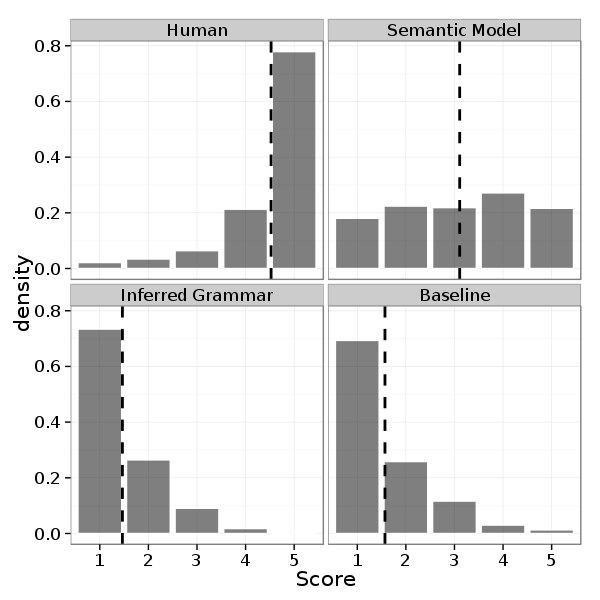
\includegraphics[height=5cm]{results/histogram_resultsByModel} 
    }}%
    \qquad
    \subfloat[Performance of each model and smoothing method]{{\label{fig:hist2}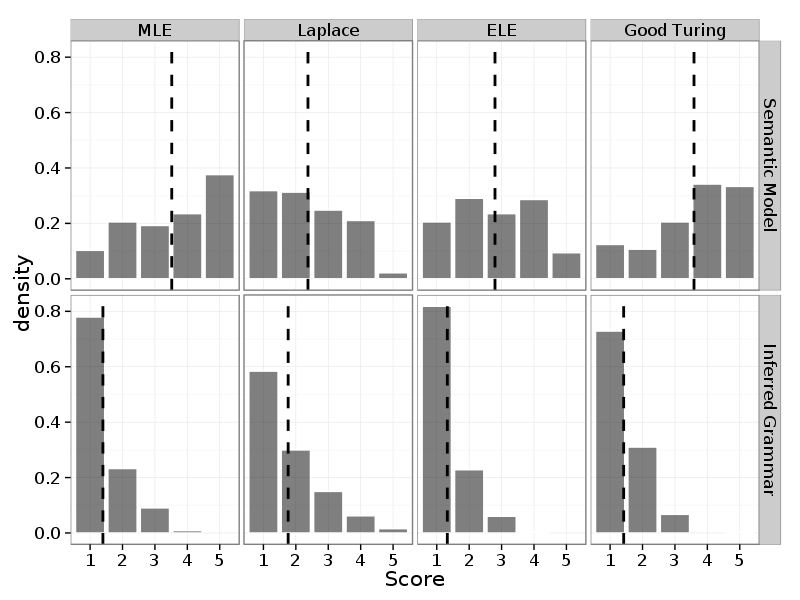
\includegraphics[height=5cm]{results/histogram_resultsByModelAndSmootingMethod} 
    }}%
    \caption{Density histograms of model scores in the perception test. Dotted lines represent means.}%
    \label{fig:histograms}%
\end{figure}

\begin{figure}%
    \centering
    \subfloat[Performance of each model as well as the real and baseline sentences]{{\label{fig:boxplot1}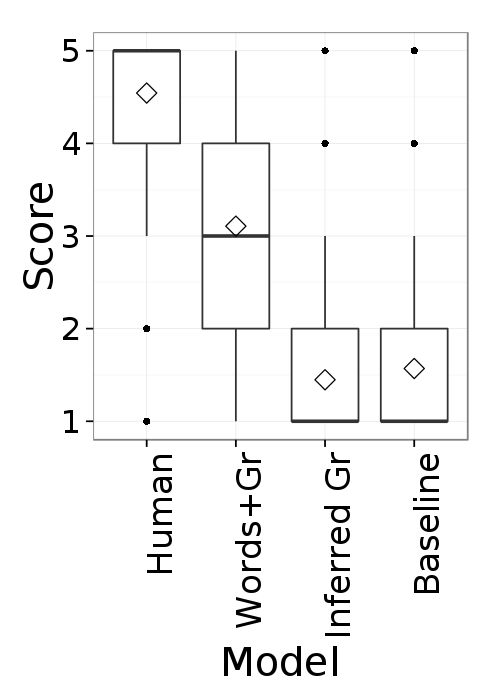
\includegraphics[height=6.2cm]{results/boxplot_resultsByModel} }}%    
    \qquad
    \subfloat[Performance of each model and smoothing method]{{\label{fig:boxplot2}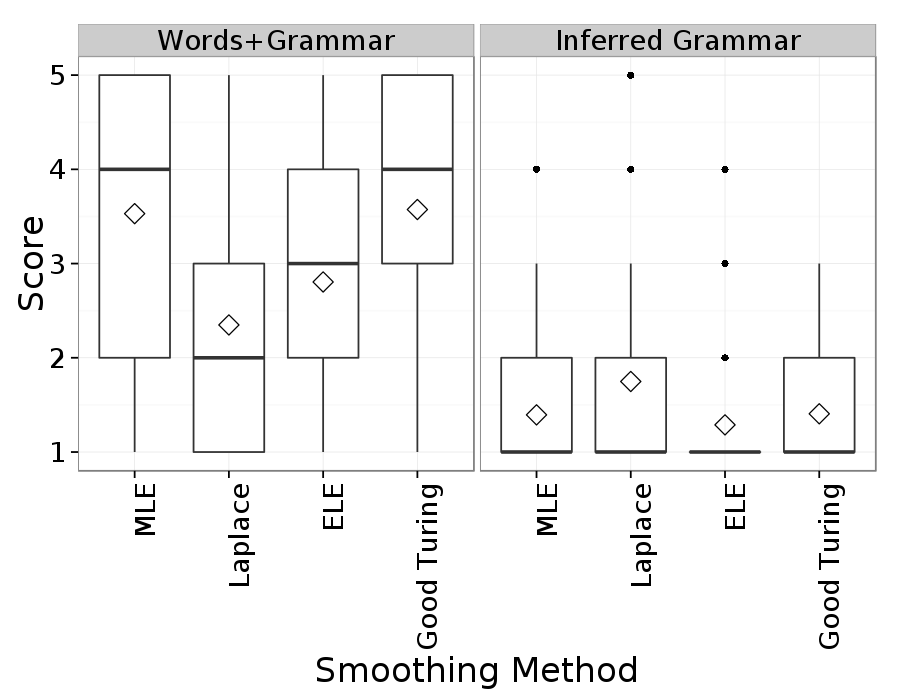
\includegraphics[height=6cm]{results/boxplot_resultsByModelAndSmoothing} }}%
    \qquad
    \caption{Boxplots of model scores in the perception test. Diamonds represent   means.}%
  \label{fig:boxplots}
\end{figure}

\begin{table}[]
\centering
\caption{Model performance statistics from perception test}
\label{tab:modelStats}
\begin{tabular}{@{}lllll@{}}
\toprule
Model            & Smoothing Method & Mean & Median & Mode \\ \midrule
Semantic Model   & MLE              & 3.5  & 4      & 5    \\
Semantic Model   & Laplace          & 2.4  & 2      & 1    \\
Semantic Model   & ELE              & 2.8  & 3      & 2    \\
Semantic Model   & Good Turing      & 3.6  & 4      & 4    \\
Inferred Grammar & MLE              & 1.4  & 1      & 1    \\
Inferred Grammar & Laplace          & 1.8  & 1      & 1    \\
Inferred Grammar & ELE              & 1.3  & 1      & 1    \\
Inferred Grammar & Good Turing      & 1.4  & 1      & 1    \\ \bottomrule
\end{tabular}
\end{table}

%%%%%%%%%%%%%%%%%%%%%%%%%%%%%%%%%%%%%%%%%%
%%%%%%%%%%%%%%%%%%%%%%%%%%%%%%%%%%%%%%%%%%
\subsection{Results}
\label{sec:results}
The results for the two implemented models, as detailed in section~\ref{sec:method}, were very different. The density distribution of answers can been seen in figures~\ref{fig:hist1} and~\ref{fig:hist2} which show that the results for SM* are rather evenly spread while the results for IGM* are are very skewed with most scores very low. The scores of the human and baseline sentences very high and very low, as was expected. The performance differences become even clearer in figure~\ref{fig:histograms} where we see that IGM* performs no better than the baseline, in fact the baseline has a higher mean score. Looking at the performance of different smoothing methods in figure~\ref{fig:hist2} we see that the Laplace and ELE smoothing methods result in poorer performance than MLE and Good Turing. MLE and Good Turing perform very similarly, but the Good Turing distribution is densest in the 4 and 5 scores while MLE has a greater spread. Good Turing therefore has the best performance according to the perception test.

The IGM* model performs abysmally no matter the smoothing method, with only Laplace smoothing pulling the mean score slightly up.







What answer was found to the research question; what did the study find? Was the tested hypothesis true?

%%%%%%%%%%%%%%%%%%%%%%%%%%%%%%%%%%%%%%%%%%%%%%%%%%%%%%%%%%%%%
%%%%%%%%%%%%%%%%%%%%%%%%%%%%%%%%%%%%%%%%%%%%%%%%%%%%%%%%%%%%%


\end{document}